\documentclass[12pt]{beamer}
%\documentclass[handout]{beamer}
%\usepackage{pgfpages}
%\mode<handout>{\setbeamercolor{background canvas}{bg=black!20}}
%\pgfpagesuselayout{2 on 1}[letterpaper,border shrink=5mm]
\usepackage{CJKutf8} 
\usepackage{graphics,soul,xcolor,color}
\usepackage{hyperref}
\usepackage[normalem]{ulem} % use normalem to protect \emph
%\mode<presentation>{\usetheme{Warsaw}}
\usetheme{Boadilla}
%\usetheme{CambridgeUS}
%\usetheme{Warsaw}
\usecolortheme{dolphin}
\usepackage{tikz}
\usetikzlibrary{mindmap}
\title[Reimplementing and Improving in RaceID]{Reimplementing and Improving in RaceID}
\author{Pei Lin, 66672977}
\institute[ShanghaiTech]{School of Information Science and Technology \\ShanghaiTech University}
\date{May 14, 2019}
\begin{document}

\begin{frame}
    \titlepage
\end{frame}

\begin{frame}
  \frametitle{Outline}
  \tableofcontents
\end{frame}

\AtBeginSection[]
{
\begin{frame}{Outline} \tableofcontents[currentsection]
    \end{frame}
}




\section{Introduction}
%%%%%%%%%%%%%%%%%%%%%%%%%%%%%%%
%page1
\begin{frame}{\textbf{Introduction}}

\ \ \ \  Clustering analysis has been widely applied to single cell RNA-sequencing data to discover cell types and cell states.

\
\


\ \ \ \ RaceID is published in Nature 2014 using the data from mouse intestinal which helps to discover the rare cell type.  

\end{frame}




%%%%%%%%%%%%%%%%%%%%%%%%%%%
%page2
\begin{frame}{\textbf{Introduction to RaceID}}
\ \ \ \ RaceID is programed by R and the workflow is summarized below:

\centering
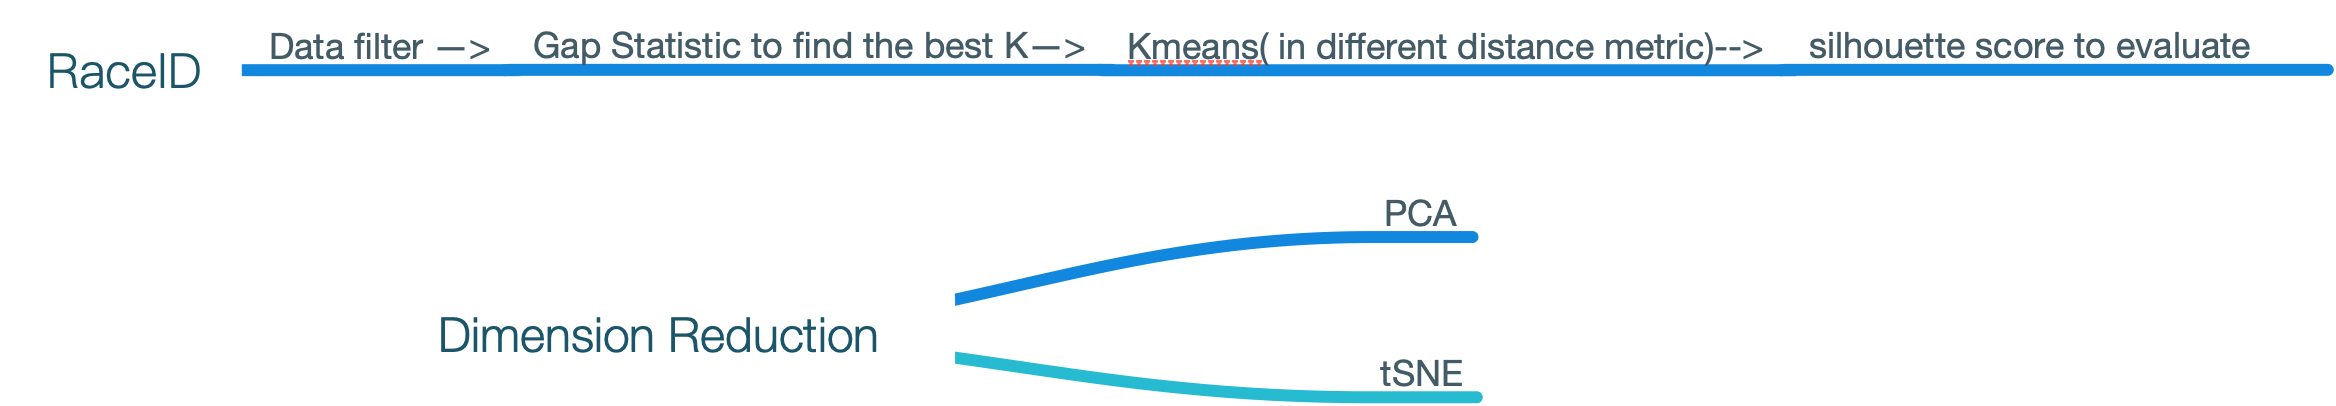
\includegraphics[scale=0.3]{fig2/workflow.png}

\end{frame}


%%%%%%%%%%%%%%%%%%%%%%%%%%%
%page3
\begin{frame}{\textbf{Introduction to My Work}}
\ \ \ \ What I have done:
\begin{itemize}
	\item \textbf{Reimplementing by Python.}
	\item \textbf{Improvement by other papers.}
	\item \textbf{Parallel programing.}
	\item \textbf{Work in another data set.}    
\end{itemize}

\end{frame}


%%%%%%%%%%%%%%%%%%%%%%%%%%%
%page4
\section{Data}
\begin{frame}{\textbf{Data Type}}
From:

1.Single-cell messenger RNA sequencing reveals rare intestinal cell types. (origin dataset)

2.Single-cell RNA-Seq profiling of human preimplantation embryos and embryonic stem cells.

\centering
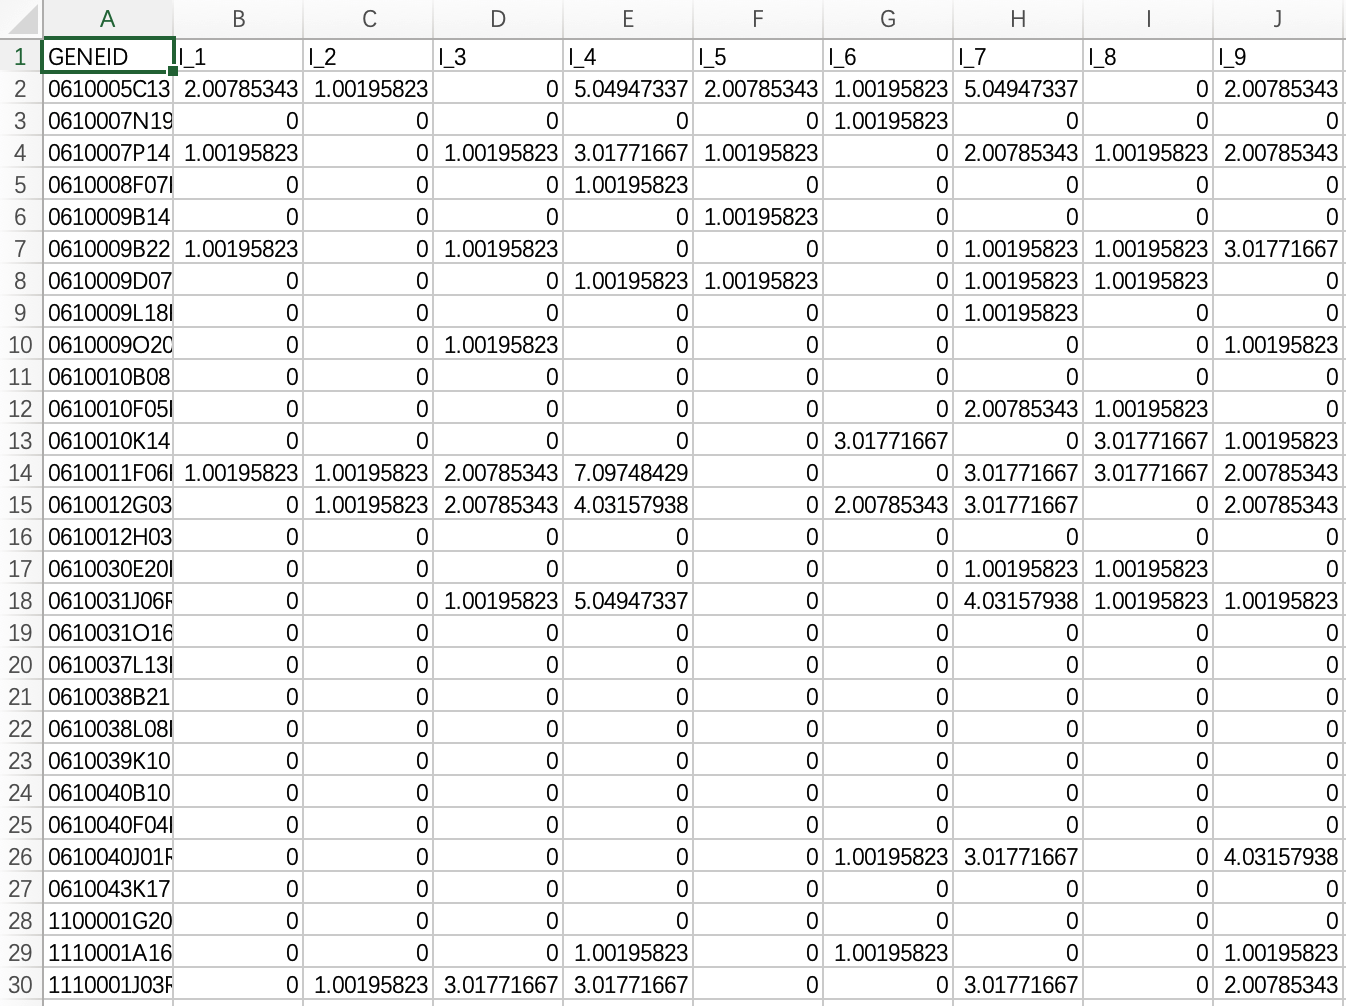
\includegraphics[scale=0.25]{fig2/data1.png}
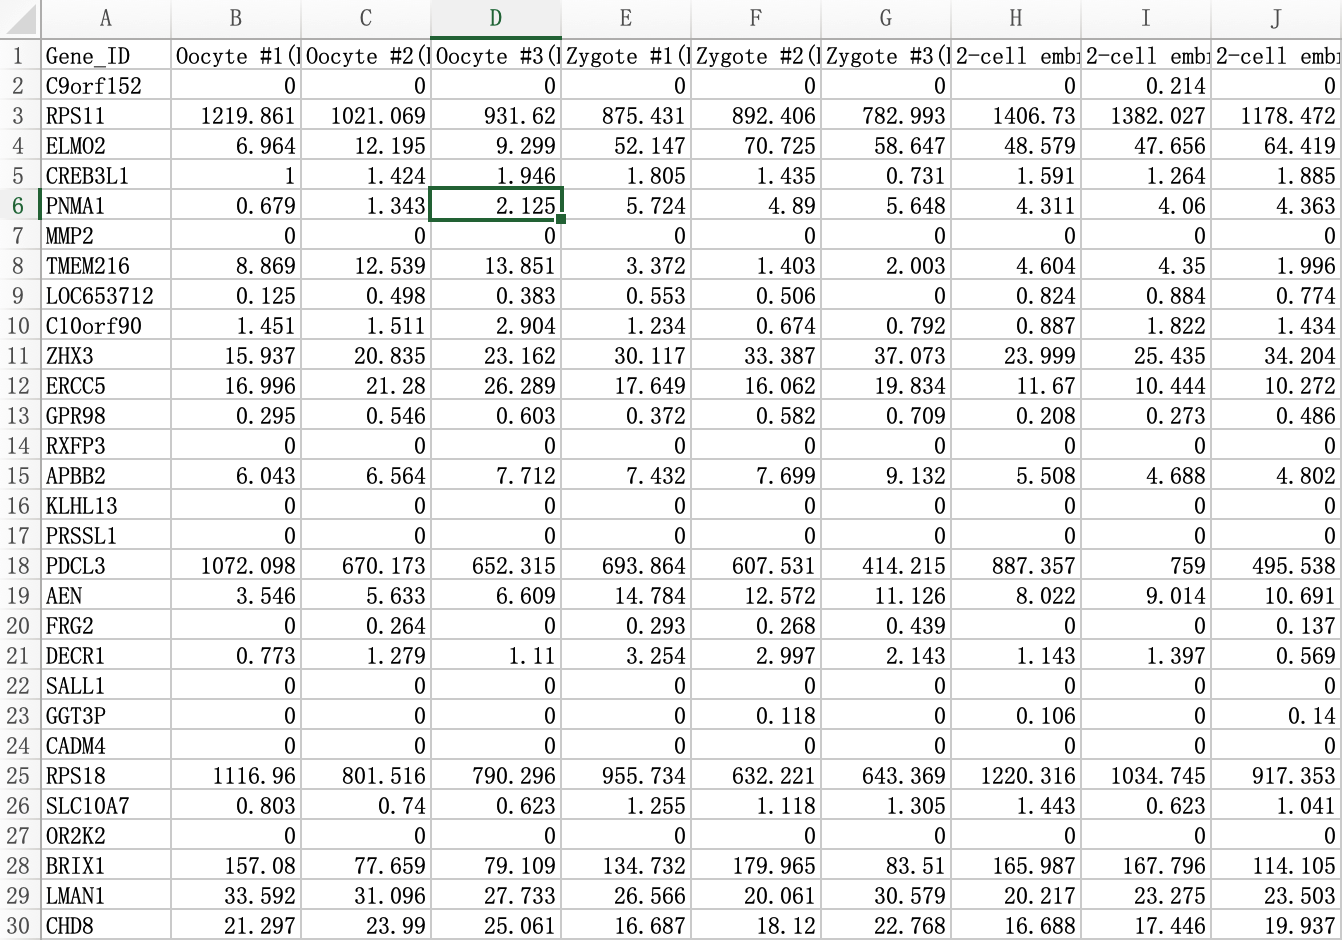
\includegraphics[scale=0.25]{fig2/data2.png}

\end{frame}


%%%%%%%%%%%%%%%%%%%%%%%%%%%
%page5
\begin{frame}{\textbf{Data Filtering \(\&\) scaling}}

For genes:
expressed in most cells(housekeeping gene)

\
\

For cells:
total expression is too low.

\
\

For scaling:

\[\frac{Gene Expression}{Mean}\rightarrow \log(Gene Expression) \]

\end{frame}






\section{Cluster}

%%%%%%%%%%%%%%%%%%%%%%%%%%%
%page6
\begin{frame}{\textbf{Kmeans}}

For Kmeans algorithm is not a convex problem, one question is how to find K and choose the initial point.

\
\

K: Calinski-Harabasz method, gap statistic

\
\

Initial point: kmeans++ method (supported by python package: sklearn.cluster)

\
\

\end{frame}

%%%%%%%%%%%%%%%%%%%%%%%%%%%
%page7
\begin{frame}{\textbf{Gap Statistic}}

Main idea is Monte Carlo method,

\[Gap_n(k)=E(logW^*)-logW\]


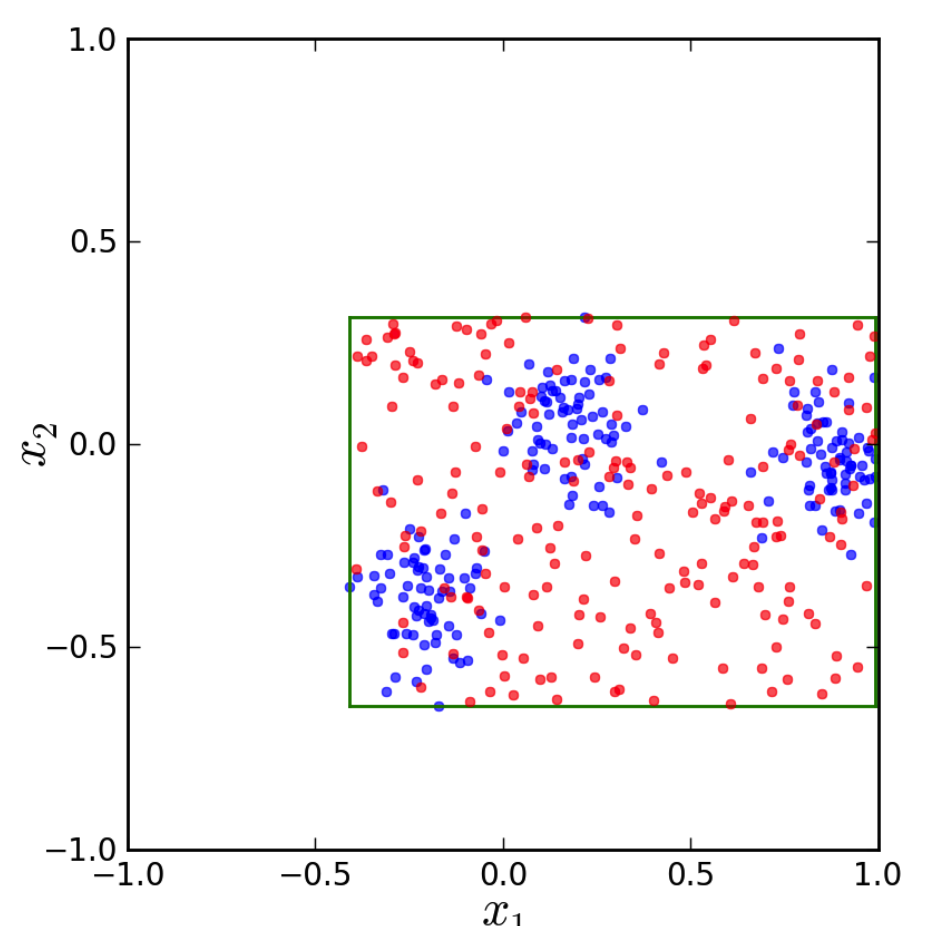
\includegraphics[scale=0.25]{fig2/gap1.png}
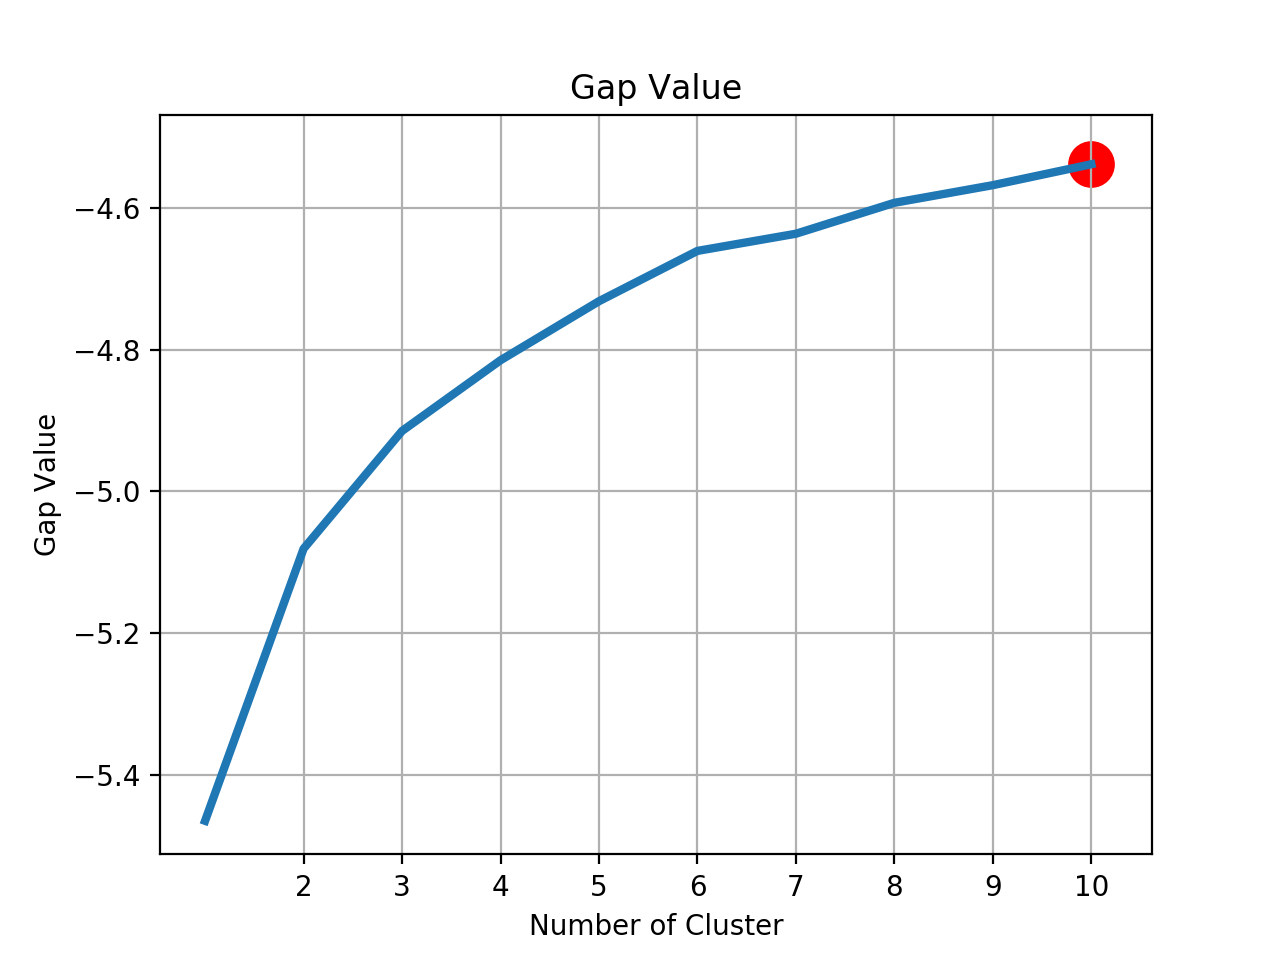
\includegraphics[scale=0.25]{fig2/gap2.png}
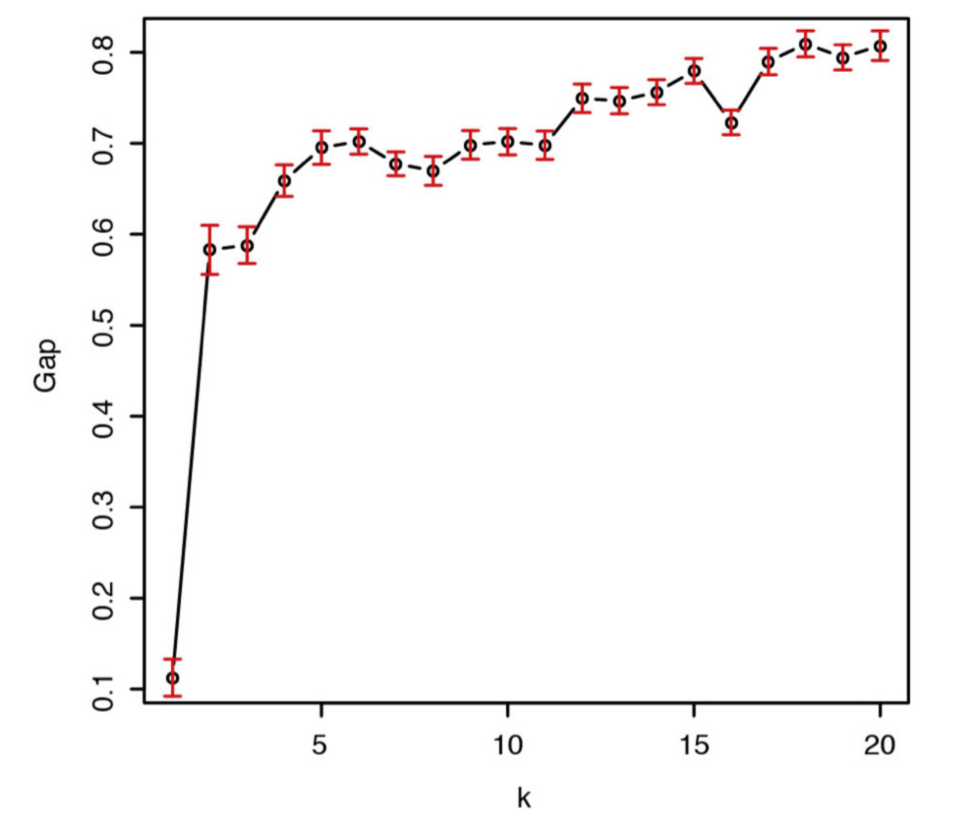
\includegraphics[scale=0.25]{fig2/gap3.png}

Because K-means is unsupervised learning, gap statistic is just a reference.
\end{frame}






\section{Dimension Reduction}
\begin{frame}{\textbf{PCA}}
\[X=U\Sigma V^T\]

PCA works for linear data.

\centering
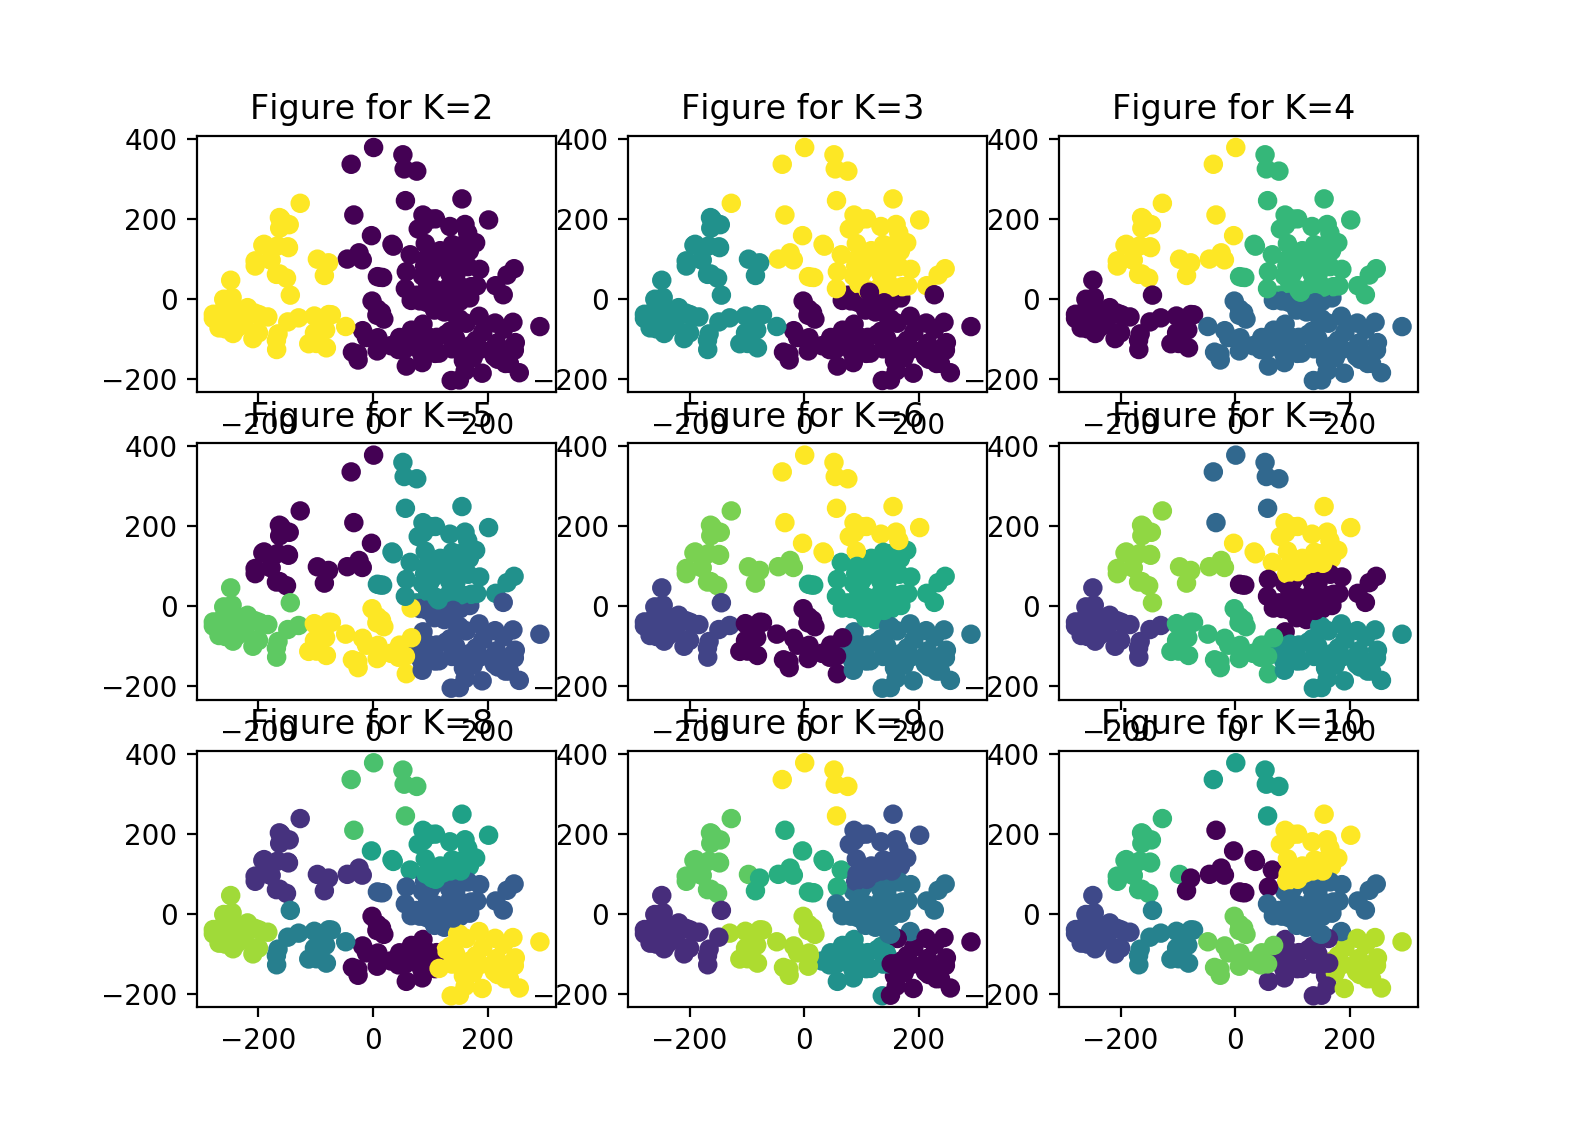
\includegraphics[scale=0.4]{fig2/pca.png}
\end{frame}




\begin{frame}{\textbf{tSNE}}

\[P_{j|i}=\frac{\exp(-||x_i-x_j||^2 /2{\sigma_i}^2)}{\sum_k \exp(-||x_i-x_k||^2 /2{\sigma_i}^2)}\]

\[q_{j|i}=\frac{\exp(-||y_i-y_j||^2)}{\sum_k \exp(-||y_i-y_k||^2 )}\]

\[C=\sum KL(P_i||Q_i)\]

tSNE usd manifold model and keep the characteristics of neighboring domain. 
\end{frame}




\begin{frame}{\textbf{tSNE}}


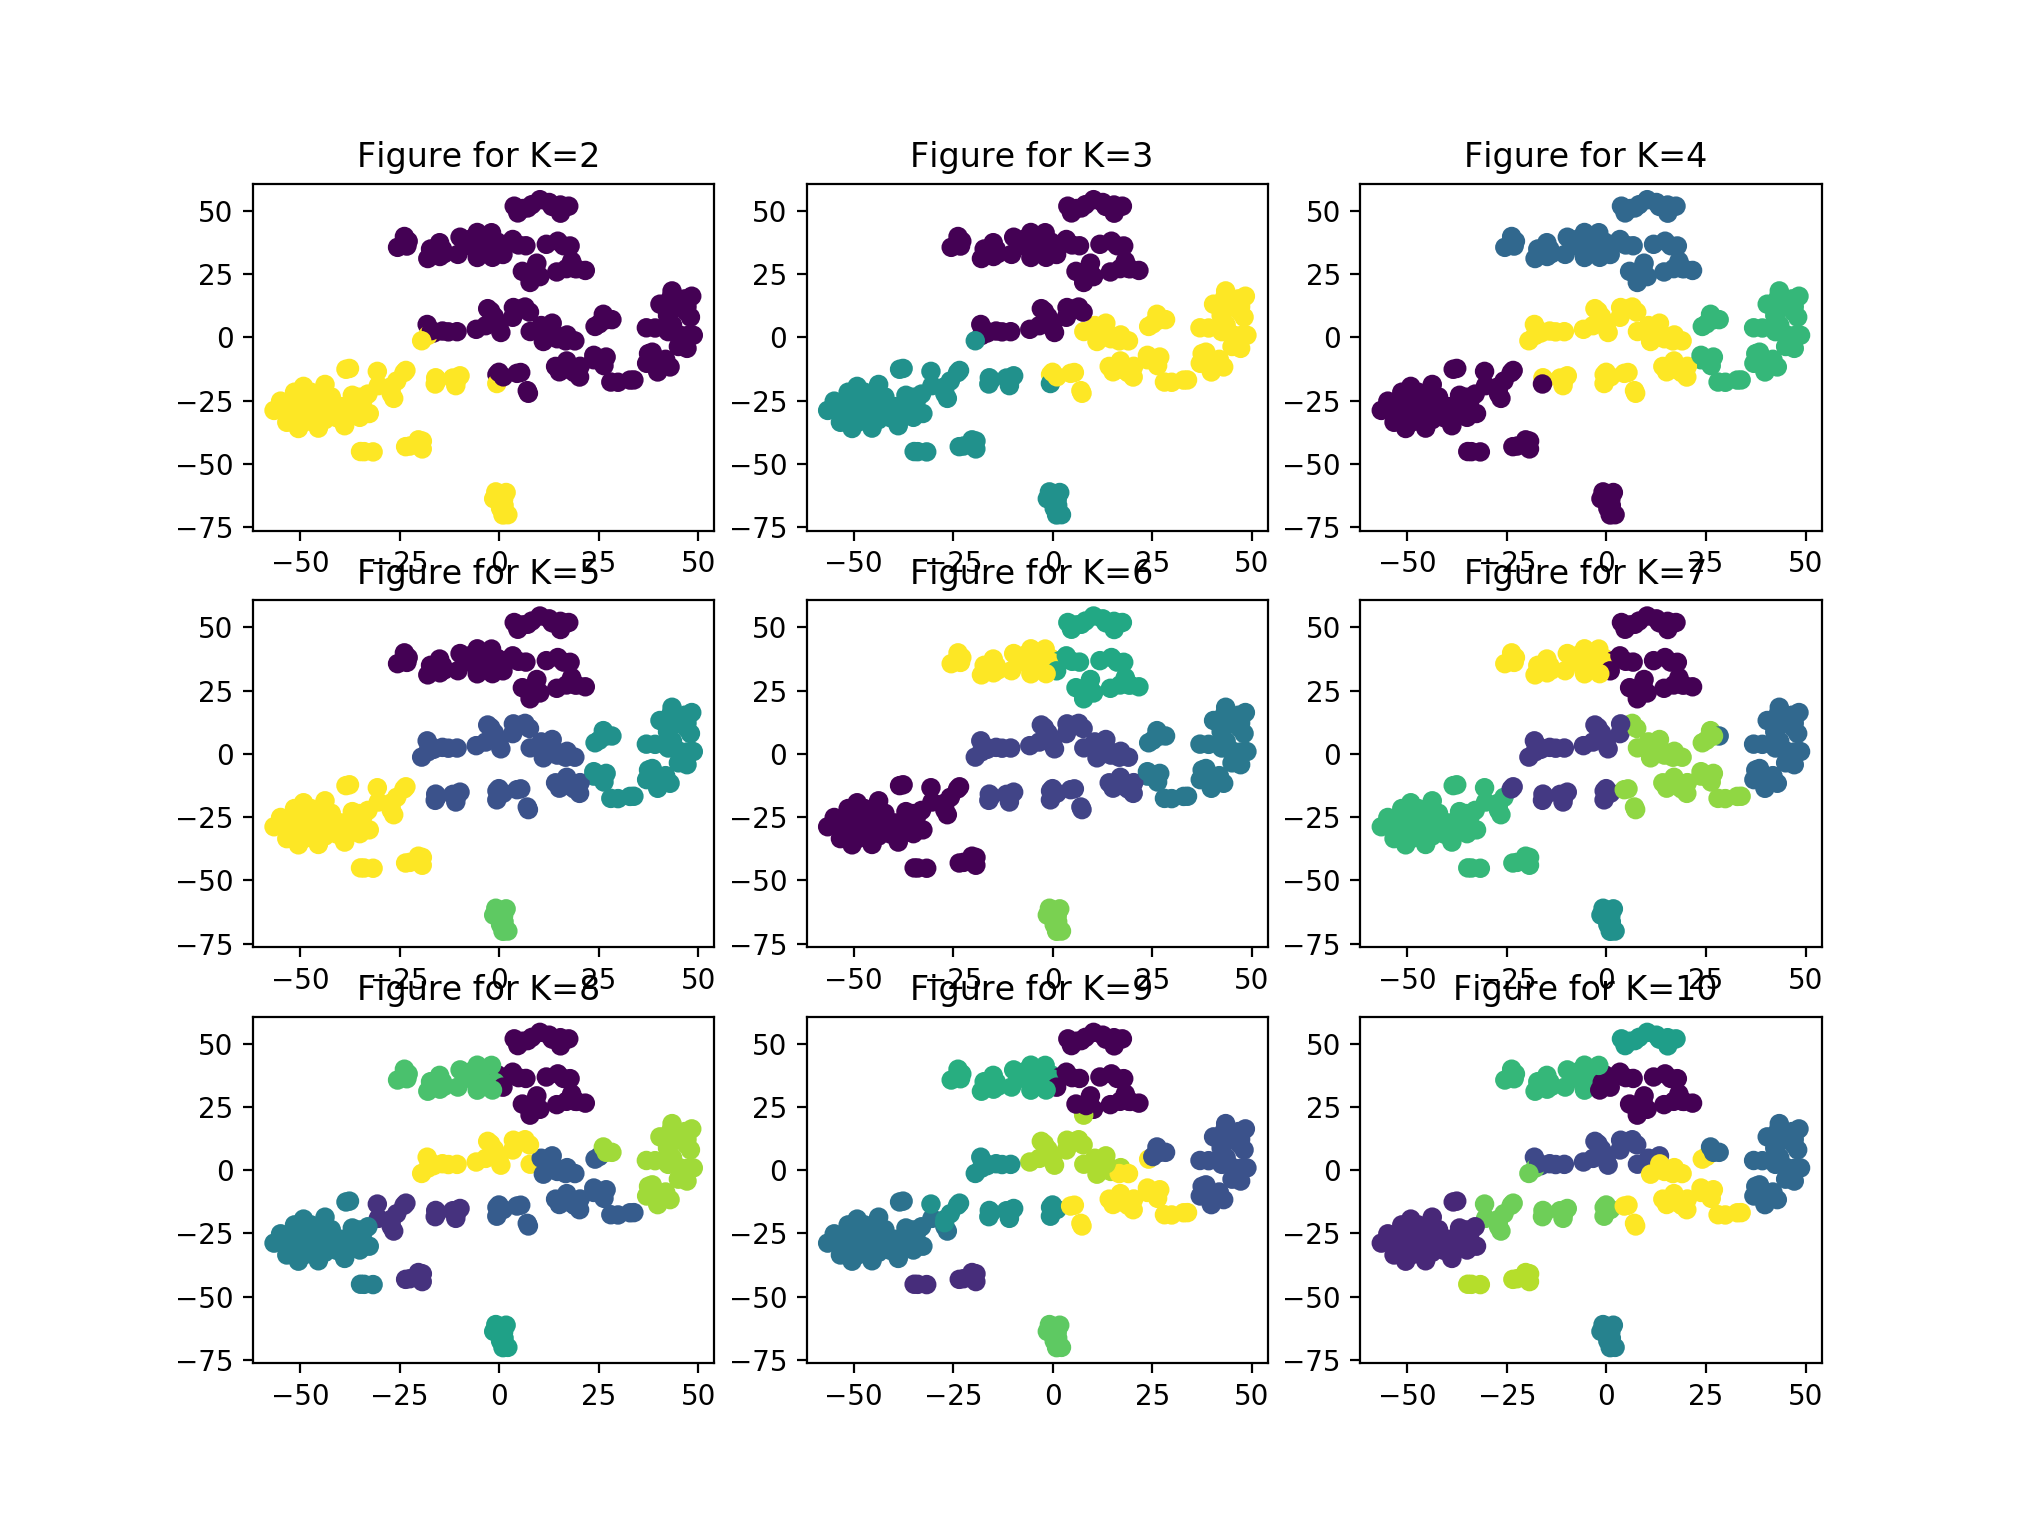
\includegraphics[scale=0.23]{fig2/tSNE.png}
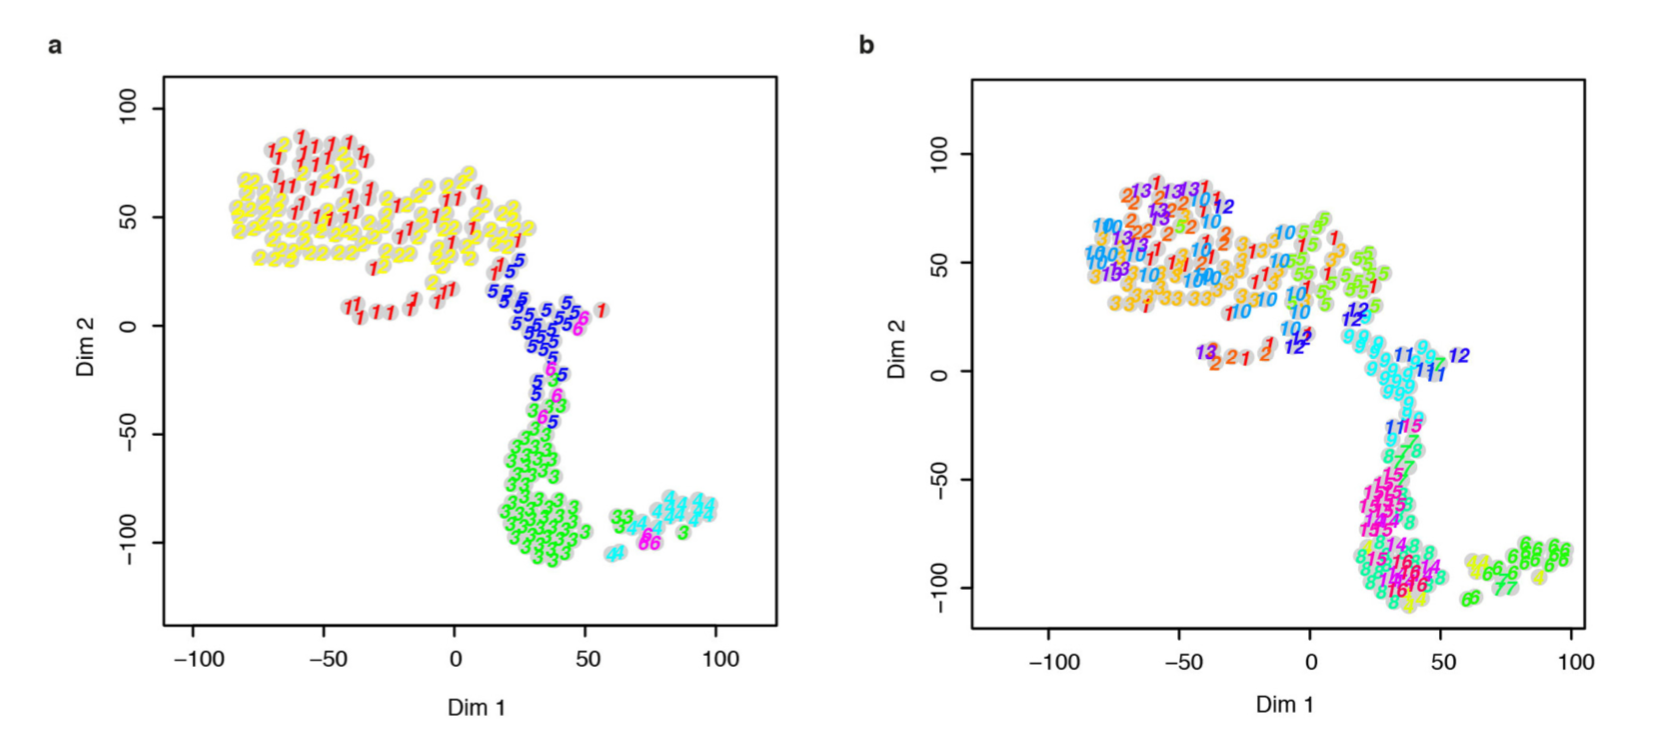
\includegraphics[scale=0.23]{fig2/tSNE2.png}
\end{frame}




\section{Parallel Programing }

\begin{frame}{Multi-thread}
Map reduce, Spark, Openmp are popular in parallel programing.

Use 10 threads to accelerating the clustering
\[MeanSpeedUp=49\%\] 

Amdahl's Law

\
\

\centering
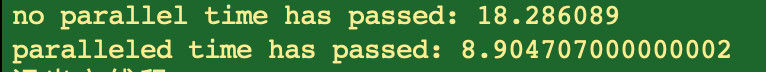
\includegraphics[scale=0.6]{fig2/parallel.png}

In R, finish the same work needs 14.2576s
\end{frame}








\section{Acknowledgment}
\begin{frame}{\textbf{Reference}}

[1]Single-cell messenger RNA sequencing reveals rare intestinal cell types, Dominic Gru, Anna Lyubimova, Lennart Kester

[2]Single-cell RNA-Seq profiling of human preimplantation embryos and embryonic stem cells, Liying Yan, Mingyu Yang, Hongshan Guo, Lu Yang

[3]Estimating the number of clusters in a data set via gap statistic, Robert Tibshirani, Guenther Weather

[4]Visualizing data using t-SNE, Laurens van der Maaten, Geoffery Hinton
\end{frame}




\bibliographystyle{IEEEtran}
\bibliography{Reference}



\begin{frame}{\textbf{}}
\centering
Thank You.
\end{frame}



\end{document}
